\section{Forecasting results}

\subsection{So sánh không impute và có impute}

So sánh quan trọng nhất là giữa observed-sales forecasting và recovered-demand forecasting. Observed-sales LightGBM đại diện cho hướng không xử lý stockout trong target. Recovered-demand LightGBM đại diện cho hướng có recovery/imputation. Khi đánh giá trên recovered latent demand proxy, WAPE giảm từ 24.42\% xuống 20.28\%. Điều này cho thấy stockout-aware recovery giúp giảm under-forecast.


\begin{table}[H]
\centering
\caption{So sánh mô hình/baseline trên recovered latent demand proxy}
\label{tab:long-main-comparison}
\resizebox{\linewidth}{!}{%
\begin{tabular}{lllllllll}
\toprule
Model & Training target & Evaluation target & RMSE & MAE & WAPE & sMAPE & WPE & N \\
\midrule
Recovered naive x7 & baseline\_no\_training & Recovered latent demand proxy & 4.3949 & 2.8080 & 0.3149 & 0.3870 & -0.0198 & 70000 \\
Recovered seasonal naive 7-day & baseline\_no\_training & Recovered latent demand proxy & 2.9113 & 1.7704 & 0.1985 & 0.2269 & -0.0614 & 70000 \\
Recovered rolling mean 14-day & baseline\_no\_training & Recovered latent demand proxy & 3.1099 & 1.8367 & 0.2060 & 0.2268 & -0.0807 & 70000 \\
Observed-sales forecasting & target\_next7\_observed\_daily & Recovered latent demand proxy & 3.6749 & 2.1780 & 0.2442 & 0.2755 & -0.1788 & 70000 \\
Observed-sales forecasting & target\_next7\_observed\_daily & Observed sales & 3.2644 & 1.7730 & 0.2206 & 0.2412 & -0.0887 & 70000 \\
Recovered-demand forecasting & target\_next7\_recovered\_daily & Recovered latent demand proxy & 3.6160 & 1.8082 & 0.2028 & 0.2135 & -0.0800 & 70000 \\
Recovered-demand forecasting & target\_next7\_recovered\_daily & Observed sales & 3.4820 & 1.7713 & 0.2204 & 0.2459 & 0.0209 & 70000 \\
Recovered seasonal-ML hybrid & seasonal\_naive\_plus\_recovered\_lightgbm\_alpha\_0.60 & Recovered latent demand proxy & 3.2106 & 1.7545 & 0.1967 & 0.2127 & -0.0726 & 70000 \\
\bottomrule
\end{tabular}
}
\end{table}



\begin{figure}[H]
    \centering
    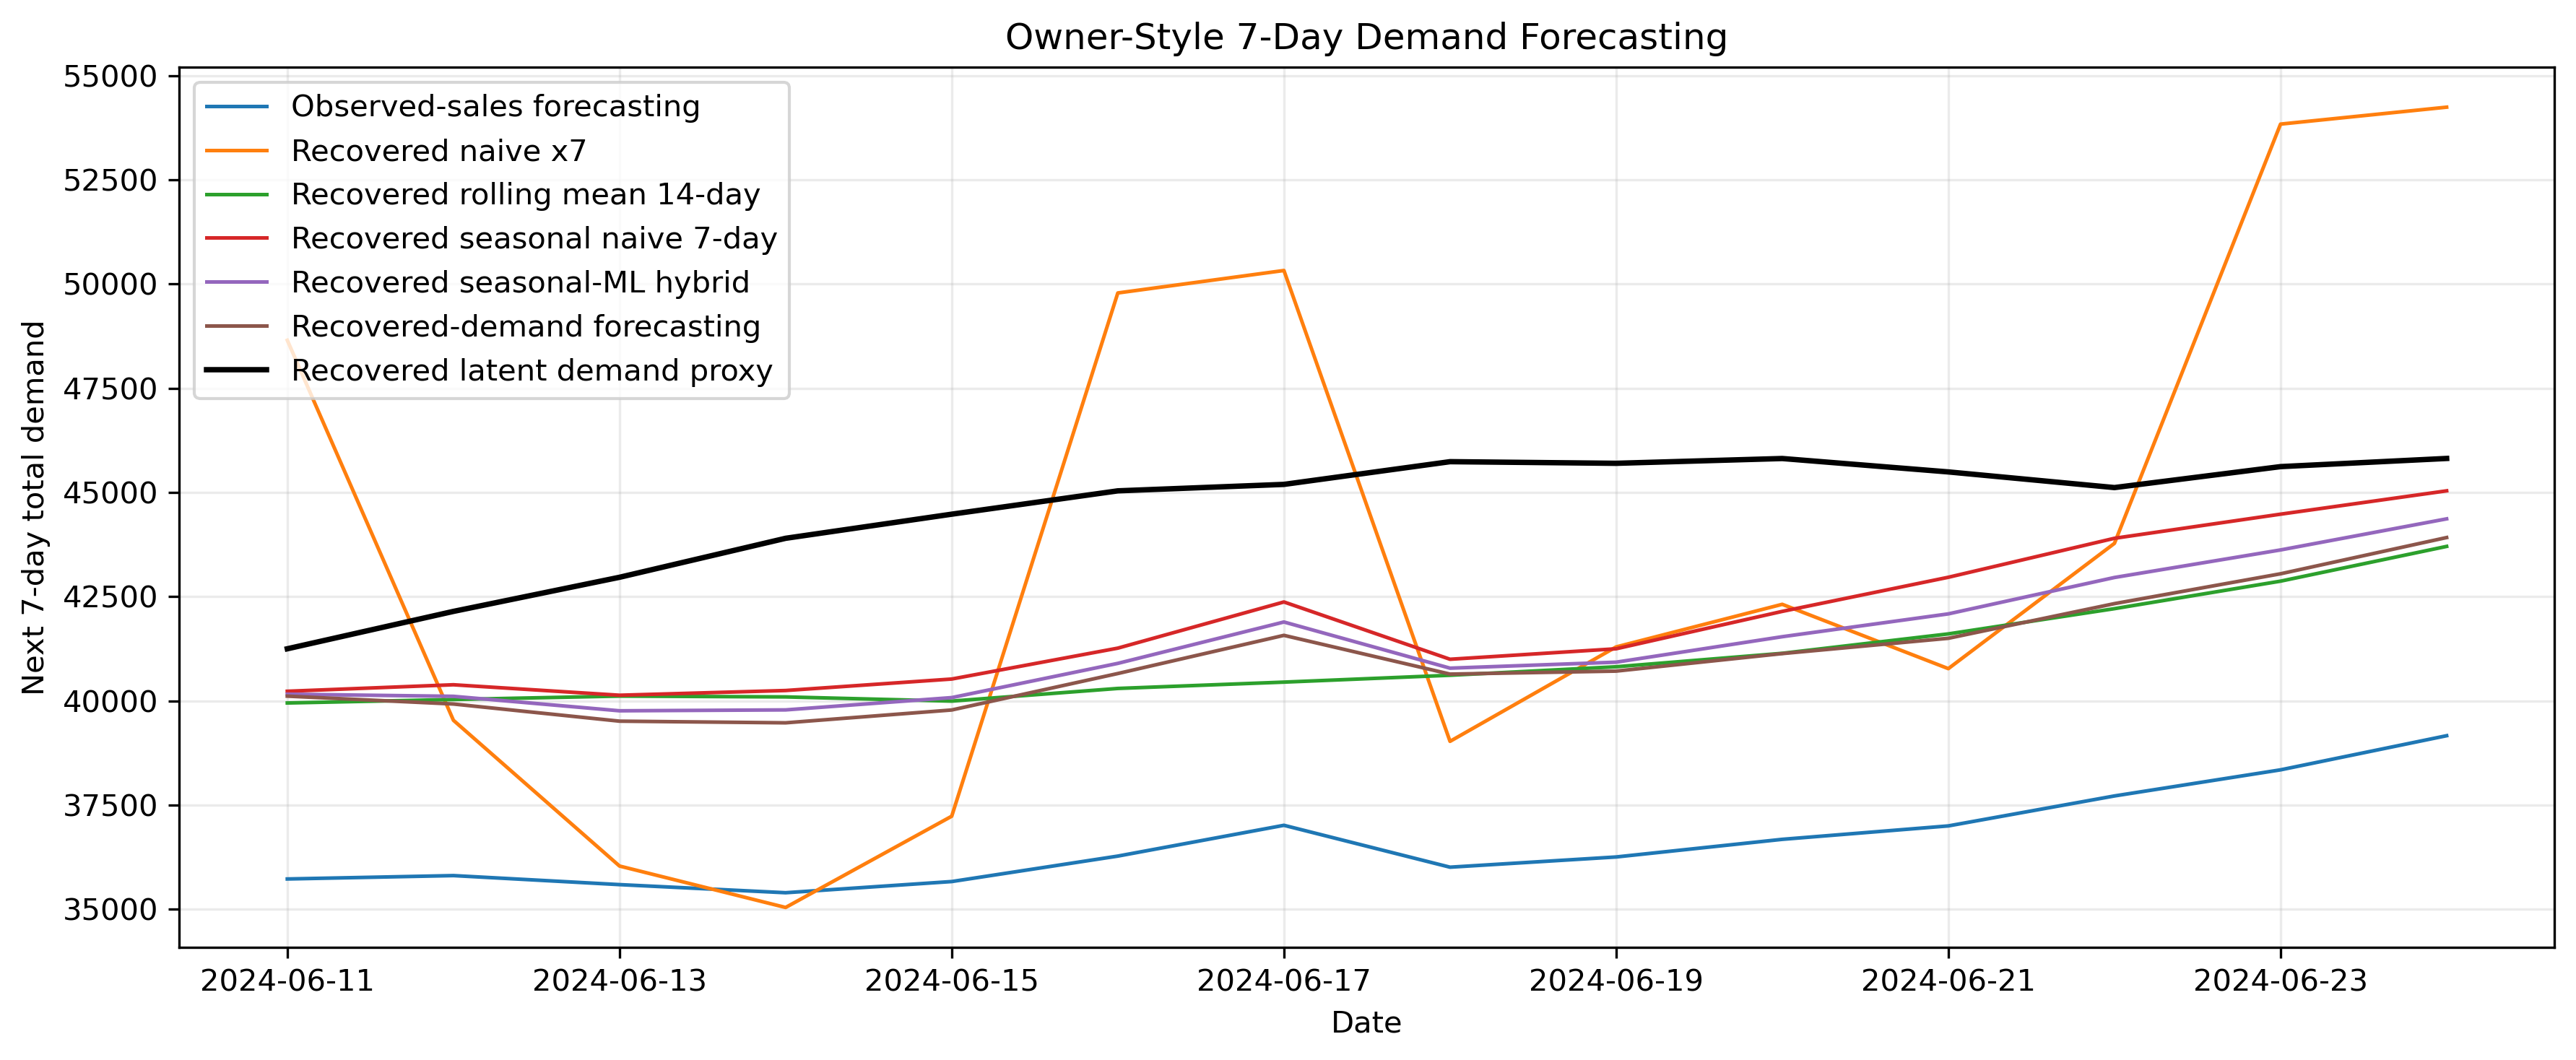
\includegraphics[width=0.92\linewidth]{figures/owner_two_stage_forecast_comparison.png}
    \caption{Forecast tổng nhu cầu 7 ngày.}
    \label{fig:long-forecast-comparison}
\end{figure}



\begin{figure}[H]
    \centering
    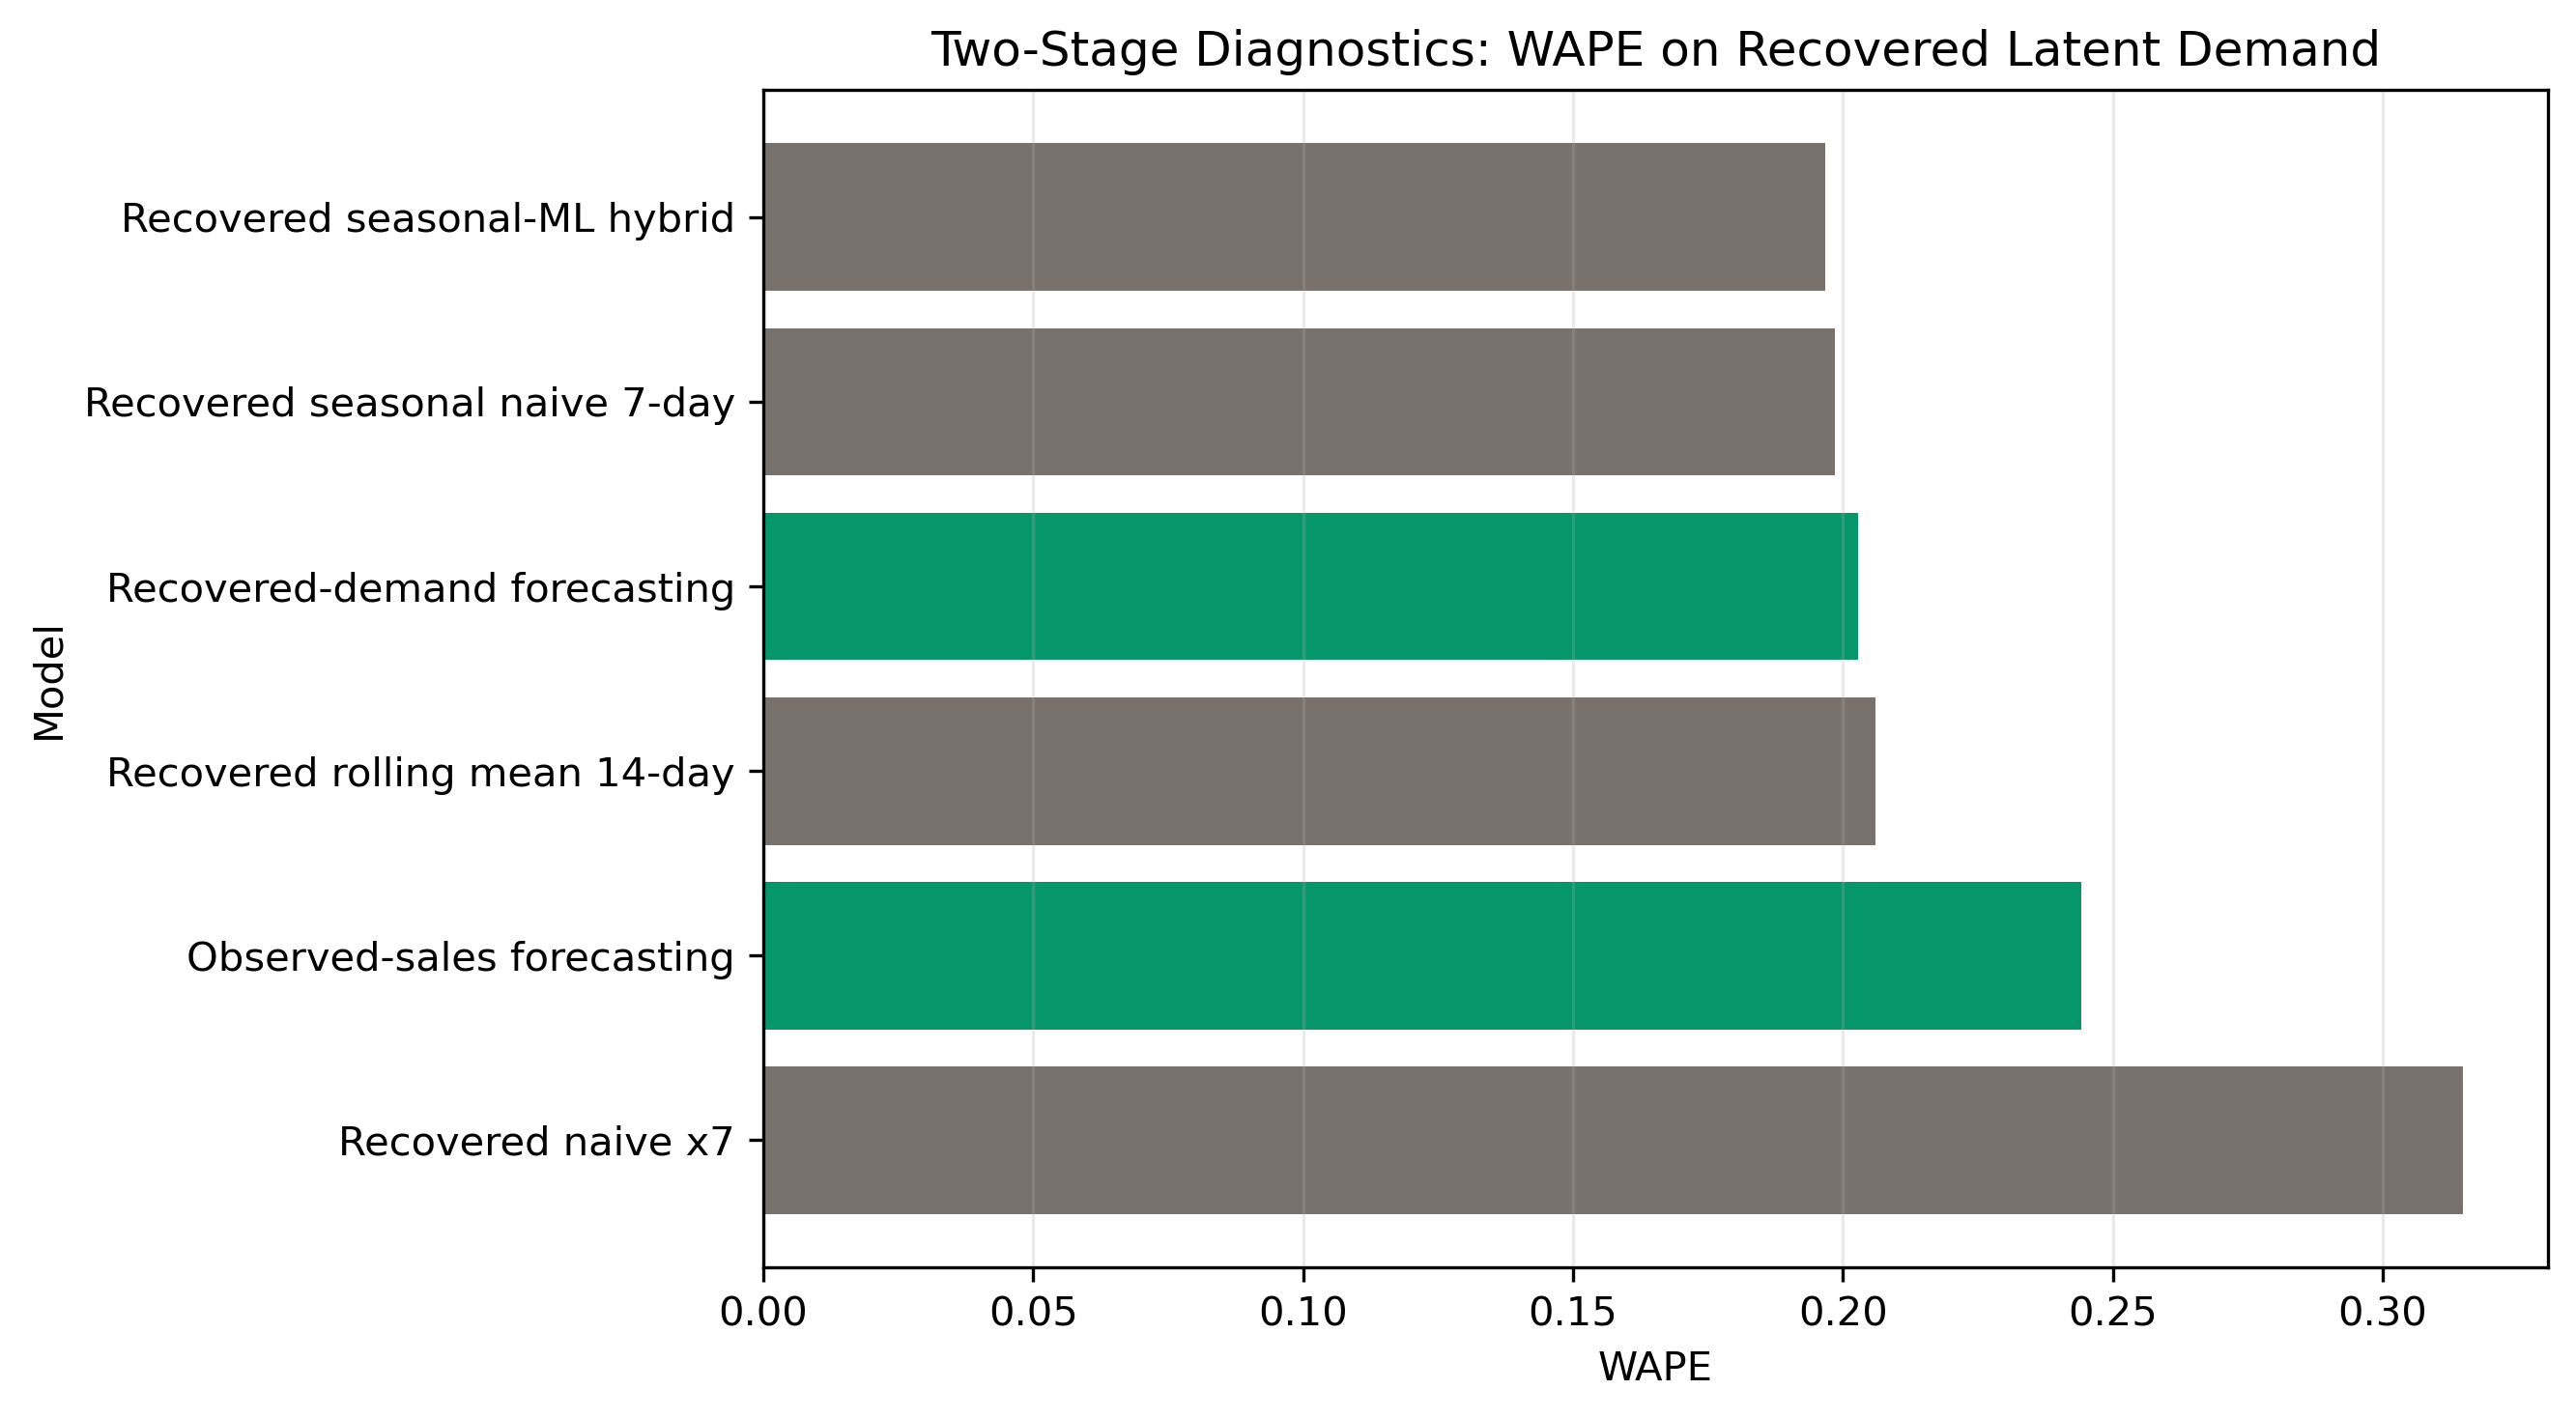
\includegraphics[width=0.92\linewidth]{figures/owner_two_stage_diagnostics_wape.png}
    \caption{WAPE của các mô hình/baseline trên recovered latent demand proxy.}
    \label{fig:long-wape}
\end{figure}


\subsection{Seasonal naive là baseline mạnh}

Seasonal naive 7-day đạt WAPE 19.85\%, tốt hơn recovered-demand LightGBM thuần. Đây không phải thất bại của ML mà là insight quan trọng: pattern tuần là thành phần nền rất mạnh. Một mô hình tốt trong bài toán này cần tôn trọng seasonality thay vì cố học lại hoàn toàn từ đầu.

\subsection{Hybrid seasonal-ML}

Hybrid seasonal-ML blend seasonal naive 7-day với recovered-demand LightGBM. Trọng số LightGBM được chọn trên validation set, không chọn bằng test. Trọng số tốt nhất hiện tại là 0.60 cho LightGBM và 0.40 cho seasonal naive. Kết quả test đạt WAPE 19.67\%, tốt nhất trong nhóm đã thử.


\begin{table}[H]
\centering
\caption{Chọn trọng số hybrid trên validation}
\label{tab:long-hybrid-blend}
\resizebox{0.80\linewidth}{!}{%
\begin{tabular}{lll}
\toprule
LightGBM weight & Seasonal naive weight & Validation WAPE \\
\midrule
0.6000 & 0.4000 & 0.1901 \\
0.5500 & 0.4500 & 0.1901 \\
0.6500 & 0.3500 & 0.1902 \\
0.5000 & 0.5000 & 0.1903 \\
0.7000 & 0.3000 & 0.1903 \\
0.4500 & 0.5500 & 0.1906 \\
0.7500 & 0.2500 & 0.1906 \\
0.4000 & 0.6000 & 0.1909 \\
0.8000 & 0.2000 & 0.1909 \\
0.3500 & 0.6500 & 0.1914 \\
\bottomrule
\end{tabular}
}
\end{table}


\subsection{Business interpretation}

Ý nghĩa của kết quả không chỉ là giảm WAPE. Nếu doanh nghiệp forecast observed sales, model có thể tiếp tục đánh giá thấp nhu cầu ở các SKU hay hết hàng. Recovery làm rõ phần demand bị ẩn, còn seasonal baseline cho thấy lịch tuần là thông tin vận hành rất quan trọng. Hybrid cuối cùng kết hợp cả hai: demand correction và weekly seasonality.

\subsection{Feature importance}

Feature importance của recovered-demand LightGBM cho thấy các lag và rolling features của recovered demand, cùng với stockout rate, là các tín hiệu quan trọng. Điều này phù hợp với trực giác: demand tương lai phụ thuộc mạnh vào mức nền gần đây, pattern tuần và mức độ kiểm duyệt bởi tồn kho.


\begin{table}[H]
\centering
\caption{Feature importance của recovered-demand LightGBM}
\label{tab:long-feature-importance}
\resizebox{0.75\linewidth}{!}{%
\begin{tabular}{ll}
\toprule
feature & importance \\
\midrule
stockout\_rate & 986 \\
recovered\_daily\_lag\_28 & 969 \\
recovered\_daily\_lag\_1 & 820 \\
recovered\_daily\_lag\_14 & 814 \\
recovered\_daily\_lag\_7 & 794 \\
recovered\_daily\_lag\_2 & 699 \\
recovered\_daily\_roll\_mean\_28 & 671 \\
recovered\_daily\_roll\_sum\_28 & 585 \\
day\_of\_week & 518 \\
recovered\_daily\_roll\_mean\_7 & 490 \\
month & 410 \\
recovered\_daily\_roll\_mean\_14 & 392 \\
recovered\_daily\_roll\_sum\_14 & 329 \\
recovered\_daily\_roll\_sum\_7 & 289 \\
is\_weekend & 23 \\
\bottomrule
\end{tabular}
}
\end{table}



\begin{figure}[H]
    \centering
    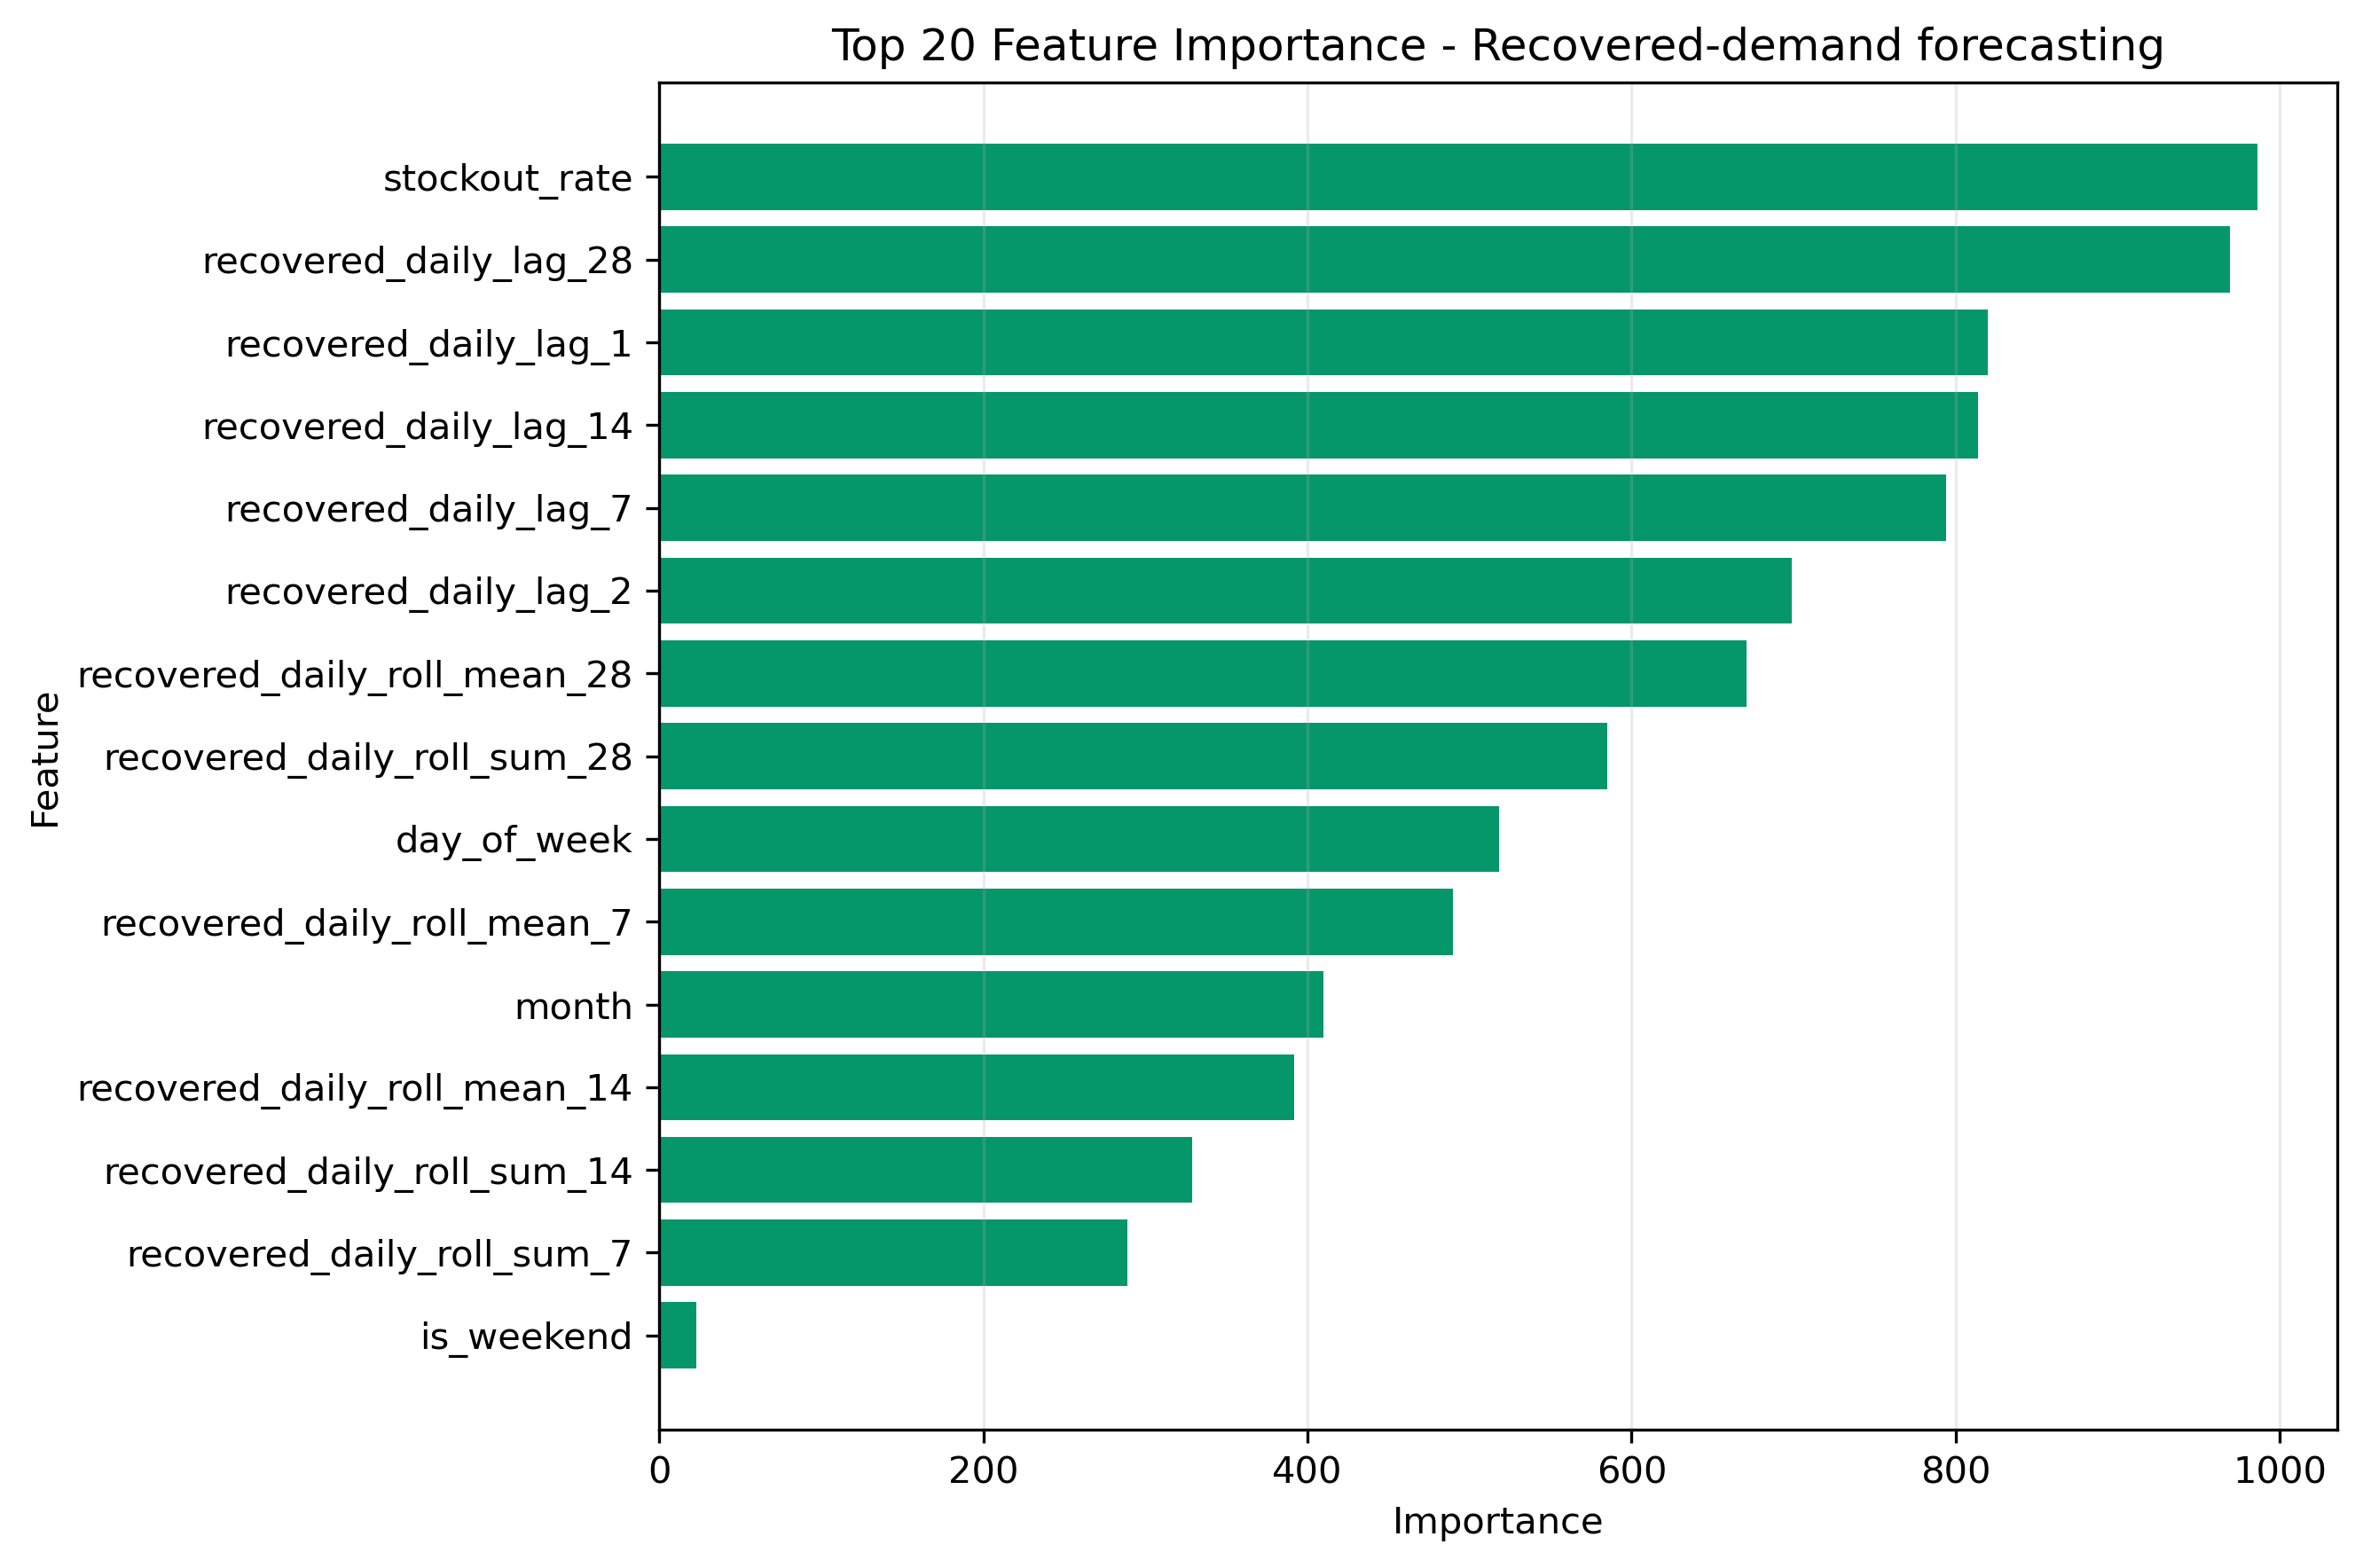
\includegraphics[width=0.78\linewidth]{figures/owner_recovereddemand_forecasting_feature_importance_top20.png}
    \caption{Top 20 feature importance.}
    \label{fig:long-feature-importance}
\end{figure}
